\documentclass[12pt]{article}

\usepackage{sbc-template}
\usepackage{graphicx,url}
\usepackage[utf8]{inputenc}

\sloppy

\title{Relatório do Projeto: ULA}
\author{Lucas da S. Inocencio}
\address{Escola Politécnica da Universidade Federal do Rio de Janeiro (UFRJ)\\
  Rio de Janeiro -- RJ -- Brasil
  \email{lucas.inocencio@Poli.ufrj.br}
}

\begin{document}

\maketitle

\section{Enunciado}

\subsection*{Objetivo}

Os alunos devem desenvolver uma ULA (Unidade Lógica e Aritmética) de 4 bits e 8 operações, das quais 4 são obrigatórias e 4 escolhidas pelo trio.

\subsection*{Especificações}

\begin{itemize}
    \item As operações a serem executadas na ULA devem selecionada por entradas de controle. O
trabalho deve ter 3 chaves externas (switchers) para controlar tais operações.
    \item Operações obrigatórias: soma, subtração em complemento de 2, incremento +1, troca de
sinal.
    \item Os alunos deverão de desenvolver um módulo auxiliar que vai servir para variar os operandos
de entrada que testarão a ALU.
    \item Elabore um relatório descrevendo a sua experiência.Os dados de entrada e o resultado da operação devem ser exibidos nos LEDs disponíveis na
placa FPGA.
    \item As saídas da ALU deve ser o resultado e as quatro flags (Zero, negativo, carry out, overflow)
que deverão ser mostrados no LEDs.
\end{itemize}


\subsection*{Funcionamento}

Os operandos de entrada são gerados por um módulo auxiliar que conterá um contator que percorrerá todos os binários representados por 4 bits. As entradas são mostradas simultaneamente nos LEDs. Em seguida, a ALU recebe os operandos e produz o resultado também mostrado no display de 7 segmentos. Além disso, a ALU gera 4 flags que são mostradas nos LEDs.

As entradas da ULA são geradas por um módulo auxiliar, um contador, parte integrante do projeto. As duas entradas são mostradas, juntamente com o resultado, nos displays de 7 segmentos disponíveis. Os LEDs são utilizados para mostrar as quatro “flags”. Os operandos vão mudando, em ordem crescente, a cada 2 segundos.

\section{Desenvolvimento}

O código fonte e documentos estão disponíveis no seguinte link: \url{https://github.com/lucas-inocencio/digital-systems}.

As 4 operações escolhidas, além das obrigatórias, foram as seguintes: XOR, Diferença absoluta, Comparador de magnitude e Calculadora de peso Hamming.

\subsection*{Soma}

A operação de soma foi projetada e implementada como vista em sala de aula. O somador de transporte antecipado (Carry-Lookahead adder) é composto por 1 gerador de soma de transporte antecipado (4 partial full adders de 1 bit), como ilustrado nas figuras abaixo:

\begin{figure}[ht]
    \centering
    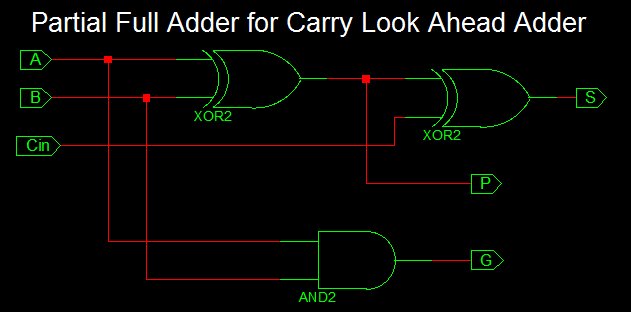
\includegraphics[scale=0.5]{partial-full-adder.png}
    \caption{Partial Full Adder}
    \label{fig:Partial Full Adder}
\end{figure}

\begin{figure}[ht]
    \centering
    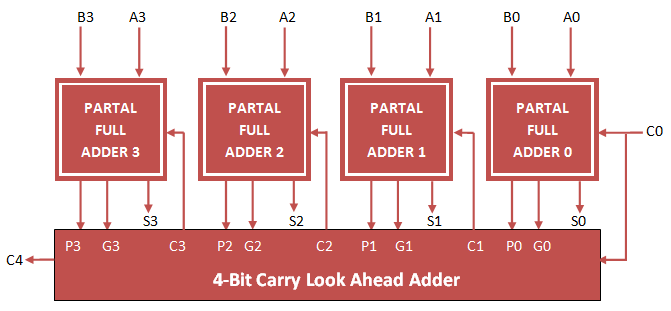
\includegraphics[scale=0.5]{cla-adder.png}
    \caption{Carry-Lookahead Adder}
    \label{fig:Carry-LookAhead Adder}
\end{figure}

\subsection*{Incremento +1}

A operação de incremento +1 consiste em utilizar o módulo de soma acima para adicionar um ao primeiro operando (o segundo é desconsiderado para esta operação).
como no trecho de codigo:

\begin{verbatim}
    carry_lookahead_adder PORT MAP(a, (OTHERS => '0'), '1', sum, carry);
\end{verbatim}

\subsection{Troca de sinal}

A operação de troca de sinal consiste em utilizar os módulos acima para realizar a inversão do sinal (em complemento de 2) do primeiro operando (um vetor de 4 bits sem sinal). Para isso, é realizada uma inversão bit-a-bit e, em seguida, um incremento de um.

\begin{verbatim}
incrementer PORT MAP(NOT (a), y, OPEN);
\end{verbatim}

\subsection*{Subtracao em complemento de 2}

A operação de subtração em complemento de 2 consiste em utilizar os módulos acima para realizar a subtração (A - B). Para isso, é feita a troca de sinal do segundo operando e uma adição com o primeiro operando, caso a soma gere carry out (ou seja, um valor maior que o esperado), o resultado é negativo e é necessário trocar o sinal do resultado final. Caso contrário, o resultado é positivo.
como no trecho de codigo:

\begin{verbatim}
    inv : inverter PORT MAP(b, b_inv);
    adder : carry_lookahead_adder PORT MAP(a, b_inv, '0', sub, sign_bit);
    inv2 : inverter PORT MAP(sub, sub_inv);
    
    PROCESS (sign_bit, sub)
    BEGIN
        IF (sign_bit = '1') THEN
            y <= sub_inv;
        ELSE
            y <= sub;
        END IF;
    END PROCESS;
\end{verbatim}

\subsection*{XOR}

A operação de ou exclusivo (XOR) consiste em realizar a operação XOR bit-a-bit.

\begin{verbatim}
    PROCESS (a, b)
    BEGIN
        FOR i IN 0 TO 3 LOOP
            y(i) <= (a(i) AND NOT b(i)) OR (NOT a(i) AND b(i));
        END LOOP;

    END PROCESS;
\end{verbatim}

\subsection*{Comparar Magnitude}

A operação de comparar magnitude consiste em determinar se o primeiro operando é igual, maior ou menor que o segundo operando, conforme visto em aula.

\begin{verbatim}
    PROCESS (a, b)
    BEGIN
        FOR i IN 3 DOWNTO 0 LOOP
            IF a(i) = '1' AND b(i) = '0' THEN
                eq <= '0'; gt <= '1'; lt <= '0';
                EXIT;
            ELSIF a(i) = '0' AND b(i) = '1' THEN
                eq <= '0'; gt <= '0'; lt <= '1';
                EXIT;
            ELSIF (a(i) = '1' AND b(i) = '1') OR (a(i) = '0' AND b(i) = '0') THEN
                eq <= '1'; gt <= '0'; lt <= '0';
            END IF;
        END LOOP;
    END PROCESS;
\end{verbatim}

\subsection*{Diferenca absoluta}

A operação de diferença absoluta utiliza o módulo comparar magnitude para realizar a subtração do maior operando pelo menor.

\begin{verbatim}
    U0 : comparator PORT MAP(a, b, equal, greater, less);
    U1 : subtractor PORT MAP(a, b, y1);
    U2 : subtractor PORT MAP(b, a, y2);

    PROCESS(equal, greater, less, a, b)
    BEGIN
        IF equal = '1' THEN
            y <= "0000";
        ELSIF greater = '1' THEN
            y <= y1;
        ELSIF less = '1' THEN
            y <= y2;
        END IF;
    END PROCESS;
\end{verbatim}

\subsection*{Calcular peso Hamming}

A operação de Hamming Weight (calcular peso de Hamming), detalhes em \url{https://en.wikipedia.org/wiki/Hamming_weight}, consiste em contar a quantidade de 1's no primeiro operando.

\begin{verbatim}
    PROCESS (a)
    BEGIN
        IF a = "0000" THEN
            y <= "00";
        ELSIF a = "0001" OR a = "0010" OR a = "0100" OR a = "1000" THEN
            y <= "01";
        ELSIF a = "1111" THEN
            y <= "11";
        ELSE
            y <= "10";
        END IF;
    END PROCESS;
\end{verbatim}

\subsection*{Contador}

\begin{verbatim}
    counter_label : PROCESS (CLOCK_50)
        VARIABLE slow_clock : INTEGER RANGE t_max DOWNTO 0 := 0;
    BEGIN
        IF (CLOCK_50'event AND CLOCK_50 = '1') THEN
            IF (slow_clock <= t_max) THEN
                slow_clock := slow_clock + 1;
            ELSE
                counter_temp <= counter_temp + 1;
                slow_clock := 0;
            END IF;
        END IF;
    END PROCESS;
    counter_out <= counter_temp;
\end{verbatim}

\subsection*{Decodificador 7 segmentos}

\begin{verbatim}
    PROCESS(bcd_in)
    BEGIN
        CASE bcd_in IS
            WHEN "0000" => seven_seg_out <= "0000001"; -- 0
            WHEN "0001" => seven_seg_out <= "1001111"; -- 1
            WHEN "0010" => seven_seg_out <= "0010010"; -- 2
            WHEN "0011" => seven_seg_out <= "0000110"; -- 3
            WHEN "0100" => seven_seg_out <= "1001100"; -- 4
            WHEN "0101" => seven_seg_out <= "0100100"; -- 5
            WHEN "0110" => seven_seg_out <= "0100000"; -- 6
            WHEN "0111" => seven_seg_out <= "0001111"; -- 7
            WHEN "1000" => seven_seg_out <= "0000000"; -- 8
            WHEN "1001" => seven_seg_out <= "0000100"; -- 9
            WHEN "1010" => seven_seg_out <= "0001000"; -- A
            WHEN "1011" => seven_seg_out <= "1100000"; -- B
            WHEN "1100" => seven_seg_out <= "0110001"; -- C
            WHEN "1101" => seven_seg_out <= "1000010"; -- D
            WHEN "1110" => seven_seg_out <= "0110000"; -- E
            WHEN "1111" => seven_seg_out <= "0111000"; -- F
            WHEN OTHERS => seven_seg_out <= "1111111"; -- OFF
        END CASE;
    END PROCESS;
\end{verbatim}


\subsection*{ULA}
A ULA consiste dos módulos acima mencionados, dois operandos de entrada de 4 bits cada (mostrados no display de 7 segmentos), 1 operando de controle de 3 bits, 1 saída de 4 bits (mostrado no display de 7 segmentos) e 4 LEDs de flags.

Foram implementados os códigos em VHDL baseados nas apresentações (slides) das aulas, no projeto e nos livros-texto "Circuit Design with VHDL" do Pedroni e "Digital Design Using VHDL: A Systems Approach" do Dally. Além disso, foram realizadas eventuais pesquisas no Google, uso do ChatGPT e GitHub Copilot.

\begin{verbatim}
    cla_adder : carry_lookahead_adder PORT MAP(a, b, '0', sum, sum_cout);
    subt : subtractor PORT MAP(a, b, sub);
    inc : incrementer PORT MAP(a, a_plus_plus, inc_cout);
    inv : inverter PORT MAP(a, a_inv);
    x0 : exor PORT MAP(a, b, xr);
    mc : comparator PORT MAP(a, b, equal, greater, less);
    abs_df : absolute_difference PORT MAP(a, b, abs_diff);
    hamming : hamming_weight_calculator PORT MAP(a, hwc);

    PROCESS(a, b, sel)
    BEGIN
        CASE sel IS
            WHEN "000" => y <= sum; -- adder
                flags(0) <= sum_cout; -- overflow
                flags(1) <= sum_cout; -- carry out
                flags(2) <= '0'; -- negative
                IF sum = "0000" THEN
                    flags(3) <= '1'; -- zero
                ELSE
                    flags(3) <= '0';
                END IF;

            WHEN "001" => y <= sub; -- subtractor
                flags(0) <= '0';
                flags(1) <= '0';
                IF b > a THEN
                    flags(2) <= '1';
                ELSE
                    flags(2) <= '0';
                END IF;
                IF sub = "0000" THEN
                    flags(3) <= '1';
                ELSE
                    flags(3) <= '0';
                END IF;

            WHEN "010" => -- incrementer
                y <= a_plus_plus;
                IF a = "1111" THEN
                    flags(0) <= '1';
                    flags(1) <= '1';
                ELSE
                    flags(0) <= '0';
                    flags(1) <= '0';
                END IF;
                IF a_plus_plus = "0000" THEN
                    flags(2) <= '1';
                ELSE
                    flags(2) <= '0';
                END IF;
                flags(3) <= '0';

            WHEN "011" => -- inverter
                y <= a_inv;
                IF a = "0000" THEN
                    flags <= "0011";
                ELSE
                    flags <= "1100";
                END IF;

            WHEN "100" => -- XOR
                y <= xr;
                flags <= "0000";

            WHEN "101" => -- comparator
                y(3) <= equal;
                y(2) <= greater;
                y(1) <= less;
                y(0) <= '0';
                flags <= "0000";

            WHEN "110" => -- absolute difference
                y <= abs_diff;
                IF abs_diff = "0000" THEN
                    flags <= "1000";
                ELSE
                    flags <= "0000";
                END IF;

            WHEN "111" => -- hamming weight calculator
                y(3) <= '0';
                y(2) <= '0';
                y(1 DOWNTO 0) <= hwc;
                IF hwc = "00" THEN
                    flags <= "1000";
                ELSE
                    flags <= "0000";
                END IF;

        END CASE;
    END PROCESS;
\end{verbatim}

\section{Testes}

Para assegurar a corretude dos códigos, foram utilizadas as ferramentas Visual Studio Code, Quartus Prime Lite e ModelSim. O compilador do Quartus foi essencial para garantir o uso da correta sintaxe do programa. Ate o momento o codigo nao foi possivel de ser testado.

\end{document}